\documentclass[12pt]{article}
\usepackage{myarticle}

\def\Sim{\mathsf{Sim}}
\def\MDL{\mathsf{MDL}}
\def\Ext{\mathsf{Ext}}

\begin{document}
\title{CS 295 \\ Blockchain \\ Final project report}
\author{Po-Chu Hsu \and Bruno Freitas}
\date{Spring 2021}
\maketitle

\section{Introduction}

In this project, we use python to implement the paxos protocol.

Our implementation consists mainly of two parts: the coordinator and the nodes. These can be run completely independently, see Usage below.

\subsection{Coordinator}

Is responsible for coordinating the nodes but is not part of the Paxos instance itself. To join the Paxos instance, every node will connect initially to the Coordinator, which will store public keys and (ip,port) pairs for the actual paxos messages between nodes. This avoids the need for each node to have a hardcoded (pkey, ip, port) for each other node, all a node needs to join Paxos is the address of the Coordinator. We use a simple TCP connection for Coord $\leftrightarrow$ Node communication and assume it is secure. Note that in deployment this should be replaced by SSL, we skip this part so as to not bother with certificates etc. At this initial connection a debug TCP socket is initialized so that nodes can send debug messages to the Coordinator. This socket is also used so that the coordinator can be used as a client, requesting nodes try to propagate a specific value. At deployment this could be used so that clients need not know any node's address, only the coordinator's.

\subsection{Node}

After connecting to the coordinator and getting the other node's information (namely verifying key, ip and UDP port) we can start the actual paxos protocol. Messages are signed using ECDSA but otherwise the protocol follows paxos using UDP so that packet dropping/delays are simply ignored by the node.

\section{Usage}

\begin{minted}{bash}
python3 paxos.py method ip port --coordip IP --coordport PORT --attack TYPE --middleware
\end{minted}

Choose a method between node (needs \textsf{--coord*}), coordinator (ignores \textsf{--coord*}), demo (takes only the \textsf{--attack} and \textsf{--middleware parameters}).

\textsf{--attack} can be used with a node or with demo, can be LIVENESS or SAFETY.

\textsf{--middleware} enables middleware to protect against both attacks


\section{Structure}

\begin{itemize}
    \item \textsf{paxos.py}: implements \textsf{\_\_main\_\_}
    \item \textsf{coordinator.py}: implements the Coordinator
    \item \textsf{node.py}: implements the Node, malicious if --attack set and using the middleware if \textsf{--middleware}
    \item \textsf{messages.py}: implements the messages that are sent Node $\leftrightarrow$ Node and Node $\leftrightarrow$ Coordinator
\end{itemize}


\section{Malicious attacks (see --attack)}

Figure \ref{fig:normal} shows a normal paxos protocol workflow. Without losing generousity, we add a commit phase at the end of the protocol. In the commit phase, the leader has to notify other replicas that he has received the majority's accept messages.

\begin{figure}[h]
    \centering
    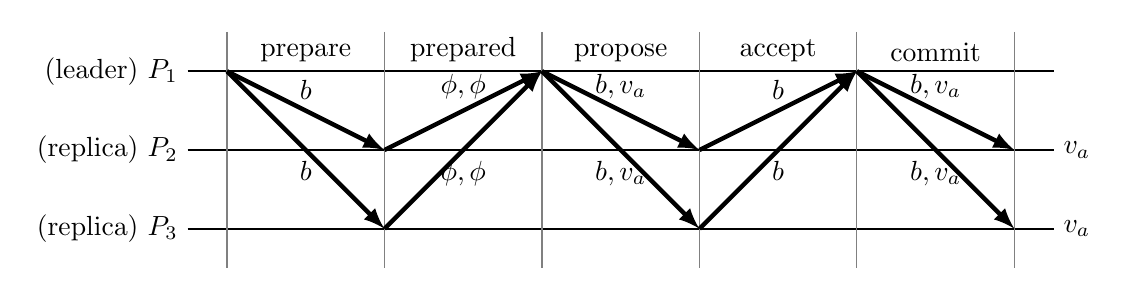
\begin{tikzpicture}[auto]
        % \tikzstyle{every node}=[font=\footnotesize];

        % horizontal line
        \draw[thick] (-0.5,-1) -- (10.5,-1);
        \draw[thick] (-0.5,-2) -- (10.5,-2);
        \draw[thick] (-0.5,-3) -- (10.5,-3);

        % vertical line
        \draw[gray] (0,-0.5) -- (0,-3.5);
        \draw[gray] (2,-0.5) -- (2,-3.5);
        \draw[gray] (4,-0.5) -- (4,-3.5);
        \draw[gray] (6,-0.5) -- (6,-3.5);
        \draw[gray] (8,-0.5) -- (8,-3.5);
        \draw[gray] (10,-0.5) -- (10,-3.5);

        % party start
        \node[anchor=east] at (-0.5,-1) {(leader) $P_1$};
        \node[anchor=east] at (-0.5,-2) {(replica) $P_2$};
        \node[anchor=east] at (-0.5,-3) {(replica) $P_3$};

        % party end
        \node[anchor=west] at (10.5,-1) {};
        \node[anchor=west] at (10.5,-2) {$v_a$};
        \node[anchor=west] at (10.5,-3) {$v_a$};

        % phase
        \node[anchor=south] at (1,-1) {prepare};
        \node[anchor=south] at (3,-1) {prepared};
        \node[anchor=south] at (5,-1) {propose};
        \node[anchor=south] at (7,-1) {accept};
        \node[anchor=south] at (9,-1) {commit};

        % prepare
        \draw[-latex, ultra thick] (0,-1) -- (2,-2) node [midway,above] {$b$};
        \draw[-latex, ultra thick] (0,-1) -- (2,-3) node [midway,below] {$b$};

        % prepared
        \draw[-latex, ultra thick] (2,-2) -- (4, -1) node [midway,above] {$\phi, \phi$};
        \draw[-latex, ultra thick] (2,-3) -- (4, -1) node [midway,below] {$\phi, \phi$};

        % propose
        \draw[-latex, ultra thick] (4,-1) -- (6,-2) node [midway,above] {$b, v_a$};
        \draw[-latex, ultra thick] (4,-1) -- (6,-3) node [midway,below] {$b, v_a$};

        % accept
        \draw[-latex, ultra thick] (6,-2) -- (8, -1) node [midway,above] {$b$};
        \draw[-latex, ultra thick] (6,-3) -- (8, -1) node [midway,below] {$b$};

        % commit
        \draw[-latex, ultra thick] (8,-1) -- (10,-2) node [midway,above] {$b, v_a$};
        \draw[-latex, ultra thick] (8,-1) -- (10,-3) node [midway,below] {$b, v_a$};
    \end{tikzpicture}
    \label{fig:normal}
    \caption{Normal situation}
\end{figure}

\subsection{SAFETY}

Assume there are $2n + 1$ nodes. Except the malicious node $M$, all other nodes are honest. Assume a fresh start.

\begin{enumerate}
    \item $M$ sends prepare(b) to all nodes.
    \item After receiving $n$ amount of prepared messages, $M$ sends propose($b$, $v_a$) to $n$ nodes and propose(b, vb) to another $n$ nodes, where $v_a \neq v_b$.
    \item As a result, $n$ nodes accept $v_a$ and $n$ nodes accept $v_b$.
\end{enumerate}


\begin{figure}[h]
    \centering
    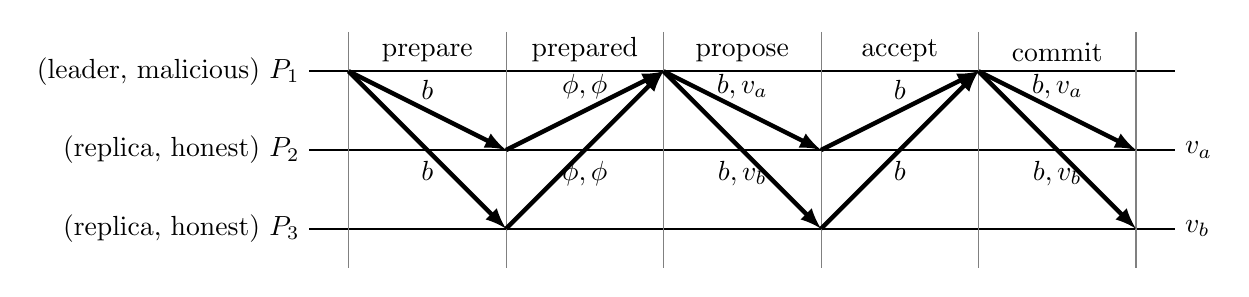
\begin{tikzpicture}[auto]
        % \tikzstyle{every node}=[font=\footnotesize];

        % horizontal line
        \draw[thick] (-0.5,-1) -- (10.5,-1);
        \draw[thick] (-0.5,-2) -- (10.5,-2);
        \draw[thick] (-0.5,-3) -- (10.5,-3);

        % vertical line
        \draw[gray] (0,-0.5) -- (0,-3.5);
        \draw[gray] (2,-0.5) -- (2,-3.5);
        \draw[gray] (4,-0.5) -- (4,-3.5);
        \draw[gray] (6,-0.5) -- (6,-3.5);
        \draw[gray] (8,-0.5) -- (8,-3.5);
        \draw[gray] (10,-0.5) -- (10,-3.5);

        % party start
        \node[anchor=east] at (-0.5,-1) {(leader, malicious) $P_1$};
        \node[anchor=east] at (-0.5,-2) {(replica, honest) $P_2$};
        \node[anchor=east] at (-0.5,-3) {(replica, honest) $P_3$};

        % party end
        \node[anchor=west] at (10.5,-1) {};
        \node[anchor=west] at (10.5,-2) {$v_a$};
        \node[anchor=west] at (10.5,-3) {$v_b$};

        % phase
        \node[anchor=south] at (1,-1) {prepare};
        \node[anchor=south] at (3,-1) {prepared};
        \node[anchor=south] at (5,-1) {propose};
        \node[anchor=south] at (7,-1) {accept};
        \node[anchor=south] at (9,-1) {commit};

        % prepare
        \draw[-latex, ultra thick] (0,-1) -- (2,-2) node [midway,above] {$b$};
        \draw[-latex, ultra thick] (0,-1) -- (2,-3) node [midway,below] {$b$};

        % prepared
        \draw[-latex, ultra thick] (2,-2) -- (4, -1) node [midway,above] {$\phi, \phi$};
        \draw[-latex, ultra thick] (2,-3) -- (4, -1) node [midway,below] {$\phi, \phi$};

        % propose
        \draw[-latex, ultra thick] (4,-1) -- (6,-2) node [midway,above] {$b, v_a$};
        \draw[-latex, ultra thick] (4,-1) -- (6,-3) node [midway,below] {$b, v_b$};

        % accept
        \draw[-latex, ultra thick] (6,-2) -- (8, -1) node [midway,above] {$b$};
        \draw[-latex, ultra thick] (6,-3) -- (8, -1) node [midway,below] {$b$};

        % commit
        \draw[-latex, ultra thick] (8,-1) -- (10,-2) node [midway,above] {$b, v_a$};
        \draw[-latex, ultra thick] (8,-1) -- (10,-3) node [midway,below] {$b, v_b$};
    \end{tikzpicture}
    \label{fig:safety}
    \caption{Safety attack}
\end{figure}

\paragraph*{Solution (implemented in the middleware)}
Nodes can broadcast every propose they receive to the other nodes. If any mismatch happens (for the same position), then we know the node is acting maliciously.


\begin{figure}[h]
    \centering
    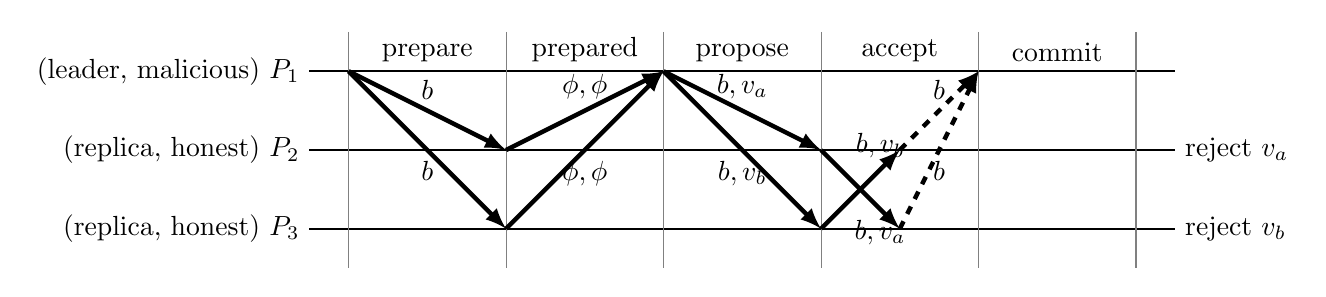
\begin{tikzpicture}[auto]
        % \tikzstyle{every node}=[font=\footnotesize];

        % horizontal line
        \draw[thick] (-0.5,-1) -- (10.5,-1);
        \draw[thick] (-0.5,-2) -- (10.5,-2);
        \draw[thick] (-0.5,-3) -- (10.5,-3);

        % vertical line
        \draw[gray] (0,-0.5) -- (0,-3.5);
        \draw[gray] (2,-0.5) -- (2,-3.5);
        \draw[gray] (4,-0.5) -- (4,-3.5);
        \draw[gray] (6,-0.5) -- (6,-3.5);
        \draw[gray] (8,-0.5) -- (8,-3.5);
        \draw[gray] (10,-0.5) -- (10,-3.5);

        % party start
        \node[anchor=east] at (-0.5,-1) {(leader, malicious) $P_1$};
        \node[anchor=east] at (-0.5,-2) {(replica, honest) $P_2$};
        \node[anchor=east] at (-0.5,-3) {(replica, honest) $P_3$};

        % party end
        \node[anchor=west] at (10.5,-1) {};
        \node[anchor=west] at (10.5,-2) {reject $v_a$};
        \node[anchor=west] at (10.5,-3) {reject $v_b$};

        % phase
        \node[anchor=south] at (1,-1) {prepare};
        \node[anchor=south] at (3,-1) {prepared};
        \node[anchor=south] at (5,-1) {propose};
        \node[anchor=south] at (7,-1) {accept};
        \node[anchor=south] at (9,-1) {commit};

        % prepare
        \draw[-latex, ultra thick] (0,-1) -- (2,-2) node [midway,above] {$b$};
        \draw[-latex, ultra thick] (0,-1) -- (2,-3) node [midway,below] {$b$};

        % prepared
        \draw[-latex, ultra thick] (2,-2) -- (4, -1) node [midway,above] {$\phi, \phi$};
        \draw[-latex, ultra thick] (2,-3) -- (4, -1) node [midway,below] {$\phi, \phi$};

        % propose
        \draw[-latex, ultra thick] (4,-1) -- (6,-2) node [midway,above] {$b, v_a$};
        \draw[-latex, ultra thick] (4,-1) -- (6,-3) node [midway,below] {$b, v_b$};

        % broadcast
        \draw[-latex, ultra thick] (6,-2) -- (7, -3) node [near end,below] {$b, v_a$};
        \draw[-latex, ultra thick] (6,-3) -- (7, -2) node [near end,above] {$b, v_b$};

        % accept
        \draw[-latex, ultra thick, dashed] (7,-2) -- (8, -1) node [midway,above] {$b$};
        \draw[-latex, ultra thick, dashed] (7,-3) -- (8, -1) node [midway,below] {$b$};

    \end{tikzpicture}
    \label{fig:safety_solution}
    \caption{Safety attack solution}
\end{figure}

\subsection{LIVENESS}

Assume there's a malicious node $M$. Everytime $M$ receives a prepare message prepare($b$), it always immediately sends a prepare message prepare($b + 1$) to all nodes and ignores the prepared messages received back. In this case, all the other nodes will not respond to prepare($b$) since they have got prepare($b + 1$).


\begin{figure}[h]
    \centering
    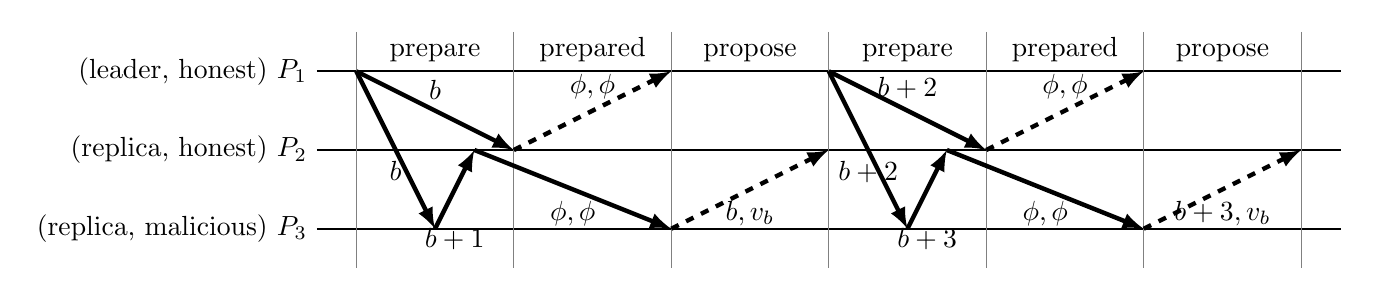
\begin{tikzpicture}[auto]
        % \tikzstyle{every node}=[font=\footnotesize];

        % horizontal line
        \draw[thick] (-0.5,-1) -- (12.5,-1);
        \draw[thick] (-0.5,-2) -- (12.5,-2);
        \draw[thick] (-0.5,-3) -- (12.5,-3);

        % vertical line
        \draw[gray] (0,-0.5) -- (0,-3.5);
        \draw[gray] (2,-0.5) -- (2,-3.5);
        \draw[gray] (4,-0.5) -- (4,-3.5);
        \draw[gray] (6,-0.5) -- (6,-3.5);
        \draw[gray] (8,-0.5) -- (8,-3.5);
        \draw[gray] (10,-0.5) -- (10,-3.5);
        \draw[gray] (12,-0.5) -- (12,-3.5);

        % party start
        \node[anchor=east] at (-0.5,-1) {(leader, honest) $P_1$};
        \node[anchor=east] at (-0.5,-2) {(replica, honest) $P_2$};
        \node[anchor=east] at (-0.5,-3) {(replica, malicious) $P_3$};

        % party end
        \node[anchor=west] at (12.5,-1) {};
        \node[anchor=west] at (12.5,-2) {};
        \node[anchor=west] at (12.5,-3) {};

        % phase
        \node[anchor=south] at (1,-1) {prepare};
        \node[anchor=south] at (3,-1) {prepared};
        \node[anchor=south] at (5,-1) {propose};
        \node[anchor=south] at (7,-1) {prepare};
        \node[anchor=south] at (9,-1) {prepared};
        \node[anchor=south] at (11,-1) {propose};

        % prepare
        \draw[-latex, ultra thick] (0,-1) -- (2,-2) node [midway,above] {$b$};
        \draw[-latex, ultra thick] (0,-1) -- (1,-3) node [midway,below] {$b$};

        \draw[-latex, ultra thick] (1,-3) -- (1.5,-2) node [midway,below=10pt] {$b + 1$};

        % prepared
        \draw[-latex, ultra thick, dashed] (2, -2) -- (4, -1) node [midway,above] {$\phi, \phi$};
        \draw[-latex, ultra thick] (1.5, -2) -- (4, -3) node [midway,below] {$\phi, \phi$};

        % propose
        \draw[-latex, ultra thick, dashed] (4, -3) -- (6, -2) node [midway,below] {$b, v_b$};

        % prepare
        \draw[-latex, ultra thick] (6,-1) -- (8,-2) node [midway,above] {$b + 2$};
        \draw[-latex, ultra thick] (6,-1) -- (7,-3) node [midway,below] {$b + 2$};

        \draw[-latex, ultra thick] (7,-3) -- (7.5,-2) node [midway,below=10pt] {$b + 3$};

        % prepared
        \draw[-latex, ultra thick, dashed] (8, -2) -- (10, -1) node [midway,above] {$\phi, \phi$};
        \draw[-latex, ultra thick] (7.5, -2) -- (10, -3) node [midway,below] {$\phi, \phi$};

        % propose
        \draw[-latex, ultra thick, dashed] (10, -3) -- (12, -2) node [midway,below] {$b + 3, v_b$};
    \end{tikzpicture}
    \label{fig:liveness}
    \caption{Liveness attack}
\end{figure}


\paragraph*{Solution (implemented in the middleware)}
Ignore a node if it tried to prepare too many times for the same position.

For demo purposes we set the number of max prepares to 3. In actual deployment we should improve this condition, possibly taking into account the timestamp of the prepares, network conditions and how many nodes there are.


\begin{figure}[h]
    \centering
    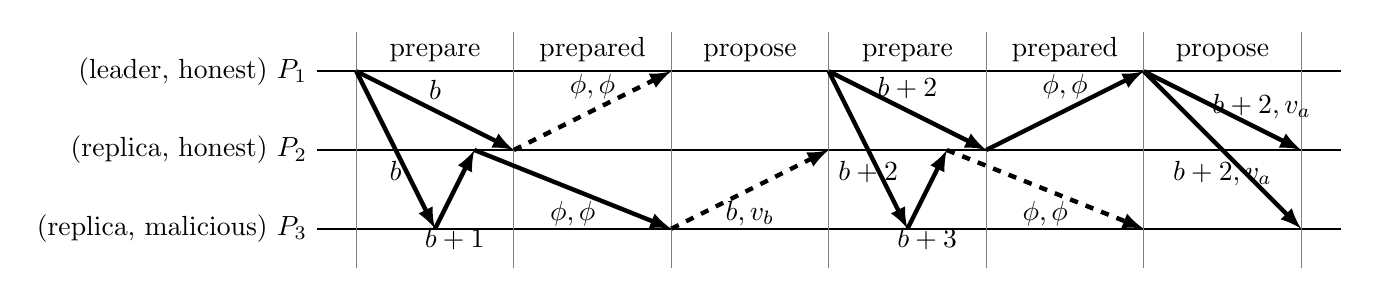
\begin{tikzpicture}[auto]
        % \tikzstyle{every node}=[font=\footnotesize];

        % horizontal line
        \draw[thick] (-0.5,-1) -- (12.5,-1);
        \draw[thick] (-0.5,-2) -- (12.5,-2);
        \draw[thick] (-0.5,-3) -- (12.5,-3);

        % vertical line
        \draw[gray] (0,-0.5) -- (0,-3.5);
        \draw[gray] (2,-0.5) -- (2,-3.5);
        \draw[gray] (4,-0.5) -- (4,-3.5);
        \draw[gray] (6,-0.5) -- (6,-3.5);
        \draw[gray] (8,-0.5) -- (8,-3.5);
        \draw[gray] (10,-0.5) -- (10,-3.5);
        \draw[gray] (12,-0.5) -- (12,-3.5);

        % party start
        \node[anchor=east] at (-0.5,-1) {(leader, honest) $P_1$};
        \node[anchor=east] at (-0.5,-2) {(replica, honest) $P_2$};
        \node[anchor=east] at (-0.5,-3) {(replica, malicious) $P_3$};

        % party end
        \node[anchor=west] at (12.5,-1) {};
        \node[anchor=west] at (12.5,-2) {};
        \node[anchor=west] at (12.5,-3) {};

        % phase
        \node[anchor=south] at (1,-1) {prepare};
        \node[anchor=south] at (3,-1) {prepared};
        \node[anchor=south] at (5,-1) {propose};
        \node[anchor=south] at (7,-1) {prepare};
        \node[anchor=south] at (9,-1) {prepared};
        \node[anchor=south] at (11,-1) {propose};

        % prepare
        \draw[-latex, ultra thick] (0,-1) -- (2,-2) node [midway,above] {$b$};
        \draw[-latex, ultra thick] (0,-1) -- (1,-3) node [midway,below] {$b$};

        \draw[-latex, ultra thick] (1,-3) -- (1.5,-2) node [midway,below=10pt] {$b + 1$};

        % prepared
        \draw[-latex, ultra thick, dashed] (2, -2) -- (4, -1) node [midway,above] {$\phi, \phi$};
        \draw[-latex, ultra thick] (1.5, -2) -- (4, -3) node [midway,below] {$\phi, \phi$};

        % propose
        \draw[-latex, ultra thick, dashed] (4, -3) -- (6, -2) node [midway,below] {$b, v_b$};

        % prepare
        \draw[-latex, ultra thick] (6,-1) -- (8,-2) node [midway,above] {$b + 2$};
        \draw[-latex, ultra thick] (6,-1) -- (7,-3) node [midway,below] {$b + 2$};

        \draw[-latex, ultra thick] (7,-3) -- (7.5,-2) node [midway,below=10pt] {$b + 3$};

        % prepared
        \draw[-latex, ultra thick] (8, -2) -- (10, -1) node [midway,above] {$\phi, \phi$};
        \draw[-latex, ultra thick, dashed] (7.5, -2) -- (10, -3) node [midway,below] {$\phi, \phi$};

        % propose
        \draw[-latex, ultra thick] (10,-1) -- (12,-2) node [near end,above] {$b + 2, v_a$};
        \draw[-latex, ultra thick] (10,-1) -- (12,-3) node [midway,below] {$b + 2, v_a$};
    \end{tikzpicture}
    \label{fig:liveness_solution}
    \caption{Liveness attack solution}
\end{figure}

\subsection{Other attacks (not implemented)}

These are some extra attacks for reference only.

\subsubsection{Liveness 2}

Malicious node send prepare($b$) where the ballot number $b$ is a maximum int then ignore all prepared messages. No other nodes can propose.

\begin{figure}[h]
    \centering
    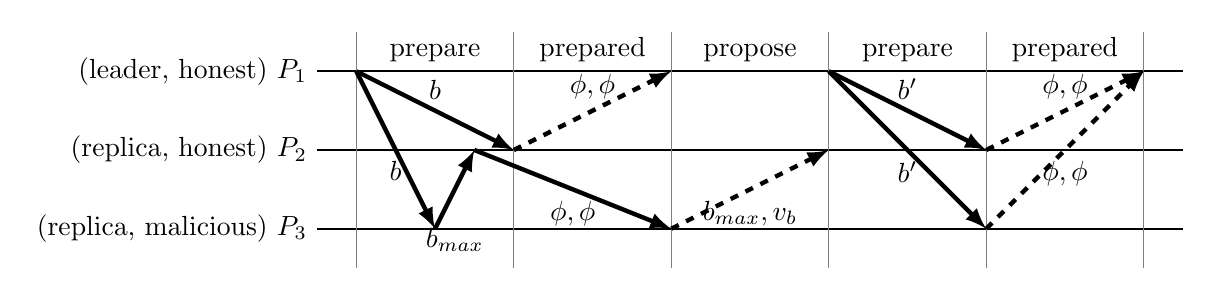
\begin{tikzpicture}[auto]
        % \tikzstyle{every node}=[font=\footnotesize];

        % horizontal line
        \draw[thick] (-0.5,-1) -- (10.5,-1);
        \draw[thick] (-0.5,-2) -- (10.5,-2);
        \draw[thick] (-0.5,-3) -- (10.5,-3);

        % vertical line
        \draw[gray] (0,-0.5) -- (0,-3.5);
        \draw[gray] (2,-0.5) -- (2,-3.5);
        \draw[gray] (4,-0.5) -- (4,-3.5);
        \draw[gray] (6,-0.5) -- (6,-3.5);
        \draw[gray] (8,-0.5) -- (8,-3.5);
        \draw[gray] (10,-0.5) -- (10,-3.5);

        % party start
        \node[anchor=east] at (-0.5,-1) {(leader, honest) $P_1$};
        \node[anchor=east] at (-0.5,-2) {(replica, honest) $P_2$};
        \node[anchor=east] at (-0.5,-3) {(replica, malicious) $P_3$};

        % party end
        \node[anchor=west] at (10.5,-1) {};
        \node[anchor=west] at (10.5,-2) {};
        \node[anchor=west] at (10.5,-3) {};

        % phase
        \node[anchor=south] at (1,-1) {prepare};
        \node[anchor=south] at (3,-1) {prepared};
        \node[anchor=south] at (5,-1) {propose};
        \node[anchor=south] at (7,-1) {prepare};
        \node[anchor=south] at (9,-1) {prepared};

        % prepare
        \draw[-latex, ultra thick] (0,-1) -- (2,-2) node [midway,above] {$b$};
        \draw[-latex, ultra thick] (0,-1) -- (1,-3) node [midway,below] {$b$};

        \draw[-latex, ultra thick] (1,-3) -- (1.5,-2) node [midway,below=10pt] {$b_{max}$};

        % prepared
        \draw[-latex, ultra thick, dashed] (2, -2) -- (4, -1) node [midway,above] {$\phi, \phi$};
        \draw[-latex, ultra thick] (1.5, -2) -- (4, -3) node [midway,below] {$\phi, \phi$};

        % propose
        \draw[-latex, ultra thick, dashed] (4, -3) -- (6, -2) node [midway,below] {$b_{max}, v_b$};

        % prepare
        \draw[-latex, ultra thick] (6,-1) -- (8,-2) node [midway,above] {$b'$};
        \draw[-latex, ultra thick] (6,-1) -- (8,-3) node [midway,below] {$b'$};

        % prepared
        \draw[-latex, ultra thick, dashed] (8, -2) -- (10, -1) node [midway,above] {$\phi, \phi$};
        \draw[-latex, ultra thick, dashed] (8, -3) -- (10, -1) node [midway,below] {$\phi, \phi$};
    \end{tikzpicture}
    \label{fig:liveness_2}
    \caption{Liveness attack 2}
\end{figure}

\paragraph*{Solution}
The difference between consecutive ballot numbers should be bounded


\begin{figure}[h]
    \centering
    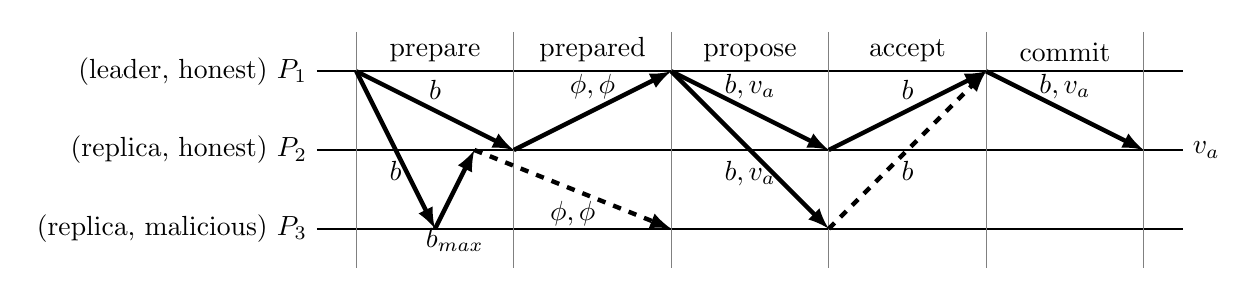
\begin{tikzpicture}[auto]
        % \tikzstyle{every node}=[font=\footnotesize];

        % horizontal line
        \draw[thick] (-0.5,-1) -- (10.5,-1);
        \draw[thick] (-0.5,-2) -- (10.5,-2);
        \draw[thick] (-0.5,-3) -- (10.5,-3);

        % vertical line
        \draw[gray] (0,-0.5) -- (0,-3.5);
        \draw[gray] (2,-0.5) -- (2,-3.5);
        \draw[gray] (4,-0.5) -- (4,-3.5);
        \draw[gray] (6,-0.5) -- (6,-3.5);
        \draw[gray] (8,-0.5) -- (8,-3.5);
        \draw[gray] (10,-0.5) -- (10,-3.5);

        % party start
        \node[anchor=east] at (-0.5,-1) {(leader, honest) $P_1$};
        \node[anchor=east] at (-0.5,-2) {(replica, honest) $P_2$};
        \node[anchor=east] at (-0.5,-3) {(replica, malicious) $P_3$};

        % party end
        \node[anchor=west] at (10.5,-1) {};
        \node[anchor=west] at (10.5,-2) {$v_a$};
        \node[anchor=west] at (10.5,-3) {};

        % phase
        \node[anchor=south] at (1,-1) {prepare};
        \node[anchor=south] at (3,-1) {prepared};
        \node[anchor=south] at (5,-1) {propose};
        \node[anchor=south] at (7,-1) {accept};
        \node[anchor=south] at (9,-1) {commit};

        % prepare
        \draw[-latex, ultra thick] (0,-1) -- (2,-2) node [midway,above] {$b$};
        \draw[-latex, ultra thick] (0,-1) -- (1,-3) node [midway,below] {$b$};

        \draw[-latex, ultra thick] (1,-3) -- (1.5,-2) node [midway,below=10pt] {$b_{max}$};

        % prepared
        \draw[-latex, ultra thick] (2, -2) -- (4, -1) node [midway,above] {$\phi, \phi$};
        \draw[-latex, ultra thick, dashed] (1.5, -2) -- (4, -3) node [midway,below] {$\phi, \phi$};

        % propose
        \draw[-latex, ultra thick] (4,-1) -- (6,-2) node [midway,above] {$b, v_a$};
        \draw[-latex, ultra thick] (4,-1) -- (6,-3) node [midway,below] {$b, v_a$};

        % accept
        \draw[-latex, ultra thick] (6,-2) -- (8, -1) node [midway,above] {$b$};
        \draw[-latex, ultra thick, dashed] (6,-3) -- (8, -1) node [midway,below] {$b$};

        % commit
        \draw[-latex, ultra thick] (8,-1) -- (10,-2) node [midway,above] {$b, v_a$};
    \end{tikzpicture}
    \label{fig:liveness_2_solution}
    \caption{Liveness attack 2 solution}
\end{figure}

\subsubsection{Liveness 3}

Instead of sending a previously prepared value (that the node received from a prepared($b, v_a$) message in reply to its prepare), malicous node send its own value $v_b$.


\begin{figure}[h]
    \centering
    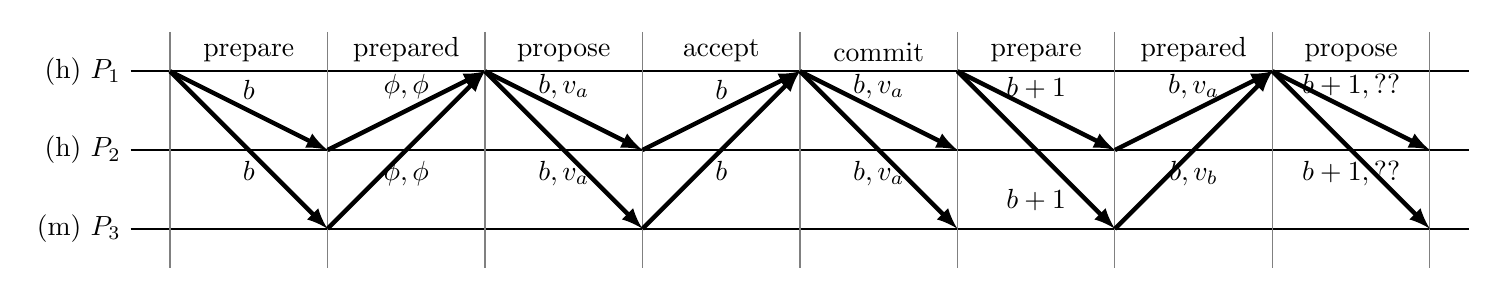
\begin{tikzpicture}[auto]
        % \tikzstyle{every node}=[font=\footnotesize];

        % horizontal line
        \draw[thick] (-0.5,-1) -- (16.5,-1);
        \draw[thick] (-0.5,-2) -- (16.5,-2);
        \draw[thick] (-0.5,-3) -- (16.5,-3);

        % vertical line
        \draw[gray] (0,-0.5) -- (0,-3.5);
        \draw[gray] (2,-0.5) -- (2,-3.5);
        \draw[gray] (4,-0.5) -- (4,-3.5);
        \draw[gray] (6,-0.5) -- (6,-3.5);
        \draw[gray] (8,-0.5) -- (8,-3.5);
        \draw[gray] (10,-0.5) -- (10,-3.5);
        \draw[gray] (12,-0.5) -- (12,-3.5);
        \draw[gray] (14,-0.5) -- (14,-3.5);
        \draw[gray] (16,-0.5) -- (16,-3.5);

        % party start
        \node[anchor=east] at (-0.5,-1) {(h) $P_1$};
        \node[anchor=east] at (-0.5,-2) {(h) $P_2$};
        \node[anchor=east] at (-0.5,-3) {(m) $P_3$};

        % party end
        \node[anchor=west] at (10.5,-1) {};
        \node[anchor=west] at (10.5,-2) {};
        \node[anchor=west] at (10.5,-3) {};

        % phase
        \node[anchor=south] at (1,-1) {prepare};
        \node[anchor=south] at (3,-1) {prepared};
        \node[anchor=south] at (5,-1) {propose};
        \node[anchor=south] at (7,-1) {accept};
        \node[anchor=south] at (9,-1) {commit};
        \node[anchor=south] at (11,-1) {prepare};
        \node[anchor=south] at (13,-1) {prepared};
        \node[anchor=south] at (15,-1) {propose};

        % prepare
        \draw[-latex, ultra thick] (0,-1) -- (2,-2) node [midway,above] {$b$};
        \draw[-latex, ultra thick] (0,-1) -- (2,-3) node [midway,below] {$b$};

        % prepared
        \draw[-latex, ultra thick] (2,-2) -- (4, -1) node [midway,above] {$\phi, \phi$};
        \draw[-latex, ultra thick] (2,-3) -- (4, -1) node [midway,below] {$\phi, \phi$};

        % propose
        \draw[-latex, ultra thick] (4,-1) -- (6,-2) node [midway,above] {$b, v_a$};
        \draw[-latex, ultra thick] (4,-1) -- (6,-3) node [midway,below] {$b, v_a$};

        % accept
        \draw[-latex, ultra thick] (6,-2) -- (8, -1) node [midway,above] {$b$};
        \draw[-latex, ultra thick] (6,-3) -- (8, -1) node [midway,below] {$b$};

        % commit
        \draw[-latex, ultra thick] (8,-1) -- (10,-2) node [midway,above] {$b, v_a$};
        \draw[-latex, ultra thick] (8,-1) -- (10,-3) node [midway,below] {$b, v_a$};

        % prepare
        \draw[-latex, ultra thick] (10,-1) -- (12,-2) node [midway,above] {$b + 1$};
        \draw[-latex, ultra thick] (10,-1) -- (12,-3) node [midway,below=10pt] {$b + 1$};

        % prepared
        \draw[-latex, ultra thick] (12,-2) -- (14, -1) node [midway,above] {$b, v_a$};
        \draw[-latex, ultra thick] (12,-3) -- (14, -1) node [midway,below] {$b, v_b$};

        % propose
        \draw[-latex, ultra thick] (14,-1) -- (16,-2) node [midway,above] {$b + 1, ??$};
        \draw[-latex, ultra thick] (14,-1) -- (16,-3) node [midway,below] {$b + 1, ??$};
    \end{tikzpicture}
    \label{fig:liveness_3}
    \caption{Liveness attack 3}
\end{figure}

\paragraph*{Solution}
When nodes send an accept($b, v$), it should be also broadcast to every other node not only to the leader. The other node's middleware will ignore any propose($b, v'$) with same ballot but $v' \neq v$.

\begin{figure}[h]
    \centering
    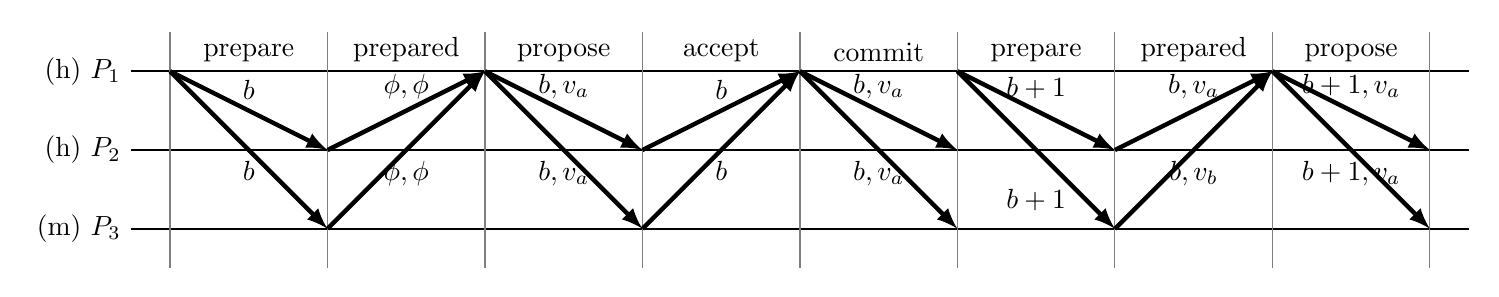
\begin{tikzpicture}[auto]
        % \tikzstyle{every node}=[font=\footnotesize];

        % horizontal line
        \draw[thick] (-0.5,-1) -- (16.5,-1);
        \draw[thick] (-0.5,-2) -- (16.5,-2);
        \draw[thick] (-0.5,-3) -- (16.5,-3);

        % vertical line
        \draw[gray] (0,-0.5) -- (0,-3.5);
        \draw[gray] (2,-0.5) -- (2,-3.5);
        \draw[gray] (4,-0.5) -- (4,-3.5);
        \draw[gray] (6,-0.5) -- (6,-3.5);
        \draw[gray] (8,-0.5) -- (8,-3.5);
        \draw[gray] (10,-0.5) -- (10,-3.5);
        \draw[gray] (12,-0.5) -- (12,-3.5);
        \draw[gray] (14,-0.5) -- (14,-3.5);
        \draw[gray] (16,-0.5) -- (16,-3.5);

        % party start
        \node[anchor=east] at (-0.5,-1) {(h) $P_1$};
        \node[anchor=east] at (-0.5,-2) {(h) $P_2$};
        \node[anchor=east] at (-0.5,-3) {(m) $P_3$};

        % party end
        \node[anchor=west] at (10.5,-1) {};
        \node[anchor=west] at (10.5,-2) {};
        \node[anchor=west] at (10.5,-3) {};

        % phase
        \node[anchor=south] at (1,-1) {prepare};
        \node[anchor=south] at (3,-1) {prepared};
        \node[anchor=south] at (5,-1) {propose};
        \node[anchor=south] at (7,-1) {accept};
        \node[anchor=south] at (9,-1) {commit};
        \node[anchor=south] at (11,-1) {prepare};
        \node[anchor=south] at (13,-1) {prepared};
        \node[anchor=south] at (15,-1) {propose};

        % prepare
        \draw[-latex, ultra thick] (0,-1) -- (2,-2) node [midway,above] {$b$};
        \draw[-latex, ultra thick] (0,-1) -- (2,-3) node [midway,below] {$b$};

        % prepared
        \draw[-latex, ultra thick] (2,-2) -- (4, -1) node [midway,above] {$\phi, \phi$};
        \draw[-latex, ultra thick] (2,-3) -- (4, -1) node [midway,below] {$\phi, \phi$};

        % propose
        \draw[-latex, ultra thick] (4,-1) -- (6,-2) node [midway,above] {$b, v_a$};
        \draw[-latex, ultra thick] (4,-1) -- (6,-3) node [midway,below] {$b, v_a$};

        % accept
        \draw[-latex, ultra thick] (6,-2) -- (8, -1) node [midway,above] {$b$};
        \draw[-latex, ultra thick] (6,-3) -- (8, -1) node [midway,below] {$b$};

        % commit
        \draw[-latex, ultra thick] (8,-1) -- (10,-2) node [midway,above] {$b, v_a$};
        \draw[-latex, ultra thick] (8,-1) -- (10,-3) node [midway,below] {$b, v_a$};

        % prepare
        \draw[-latex, ultra thick] (10,-1) -- (12,-2) node [midway,above] {$b + 1$};
        \draw[-latex, ultra thick] (10,-1) -- (12,-3) node [midway,below=10pt] {$b + 1$};

        % prepared
        \draw[-latex, ultra thick] (12,-2) -- (14, -1) node [midway,above] {$b, v_a$};
        \draw[-latex, ultra thick] (12,-3) -- (14, -1) node [midway,below] {$b, v_b$};

        % propose
        \draw[-latex, ultra thick] (14,-1) -- (16,-2) node [midway,above] {$b + 1, v_a$};
        \draw[-latex, ultra thick] (14,-1) -- (16,-3) node [midway,below] {$b + 1, v_a$};
    \end{tikzpicture}
    \label{fig:liveness_3_solution}
    \caption{Liveness attack 3 solution}
\end{figure}

\subsubsection{Safety 2}

Malicious leader sends commit after his proposal but before he receives accept messages from the majority.


\begin{figure}[h]
    \centering
    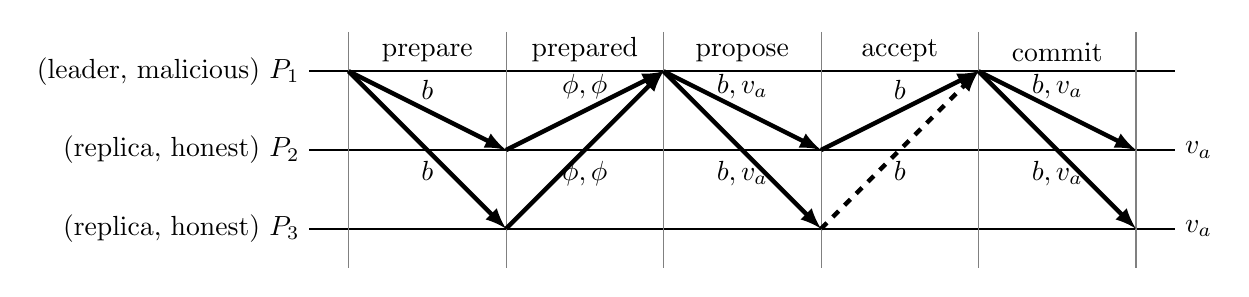
\begin{tikzpicture}[auto]
        % \tikzstyle{every node}=[font=\footnotesize];

        % horizontal line
        \draw[thick] (-0.5,-1) -- (10.5,-1);
        \draw[thick] (-0.5,-2) -- (10.5,-2);
        \draw[thick] (-0.5,-3) -- (10.5,-3);

        % vertical line
        \draw[gray] (0,-0.5) -- (0,-3.5);
        \draw[gray] (2,-0.5) -- (2,-3.5);
        \draw[gray] (4,-0.5) -- (4,-3.5);
        \draw[gray] (6,-0.5) -- (6,-3.5);
        \draw[gray] (8,-0.5) -- (8,-3.5);
        \draw[gray] (10,-0.5) -- (10,-3.5);

        % party start
        \node[anchor=east] at (-0.5,-1) {(leader, malicious) $P_1$};
        \node[anchor=east] at (-0.5,-2) {(replica, honest) $P_2$};
        \node[anchor=east] at (-0.5,-3) {(replica, honest) $P_3$};

        % party end
        \node[anchor=west] at (10.5,-1) {};
        \node[anchor=west] at (10.5,-2) {$v_a$};
        \node[anchor=west] at (10.5,-3) {$v_a$};

        % phase
        \node[anchor=south] at (1,-1) {prepare};
        \node[anchor=south] at (3,-1) {prepared};
        \node[anchor=south] at (5,-1) {propose};
        \node[anchor=south] at (7,-1) {accept};
        \node[anchor=south] at (9,-1) {commit};

        % prepare
        \draw[-latex, ultra thick] (0,-1) -- (2,-2) node [midway,above] {$b$};
        \draw[-latex, ultra thick] (0,-1) -- (2,-3) node [midway,below] {$b$};

        % prepared
        \draw[-latex, ultra thick] (2,-2) -- (4, -1) node [midway,above] {$\phi, \phi$};
        \draw[-latex, ultra thick] (2,-3) -- (4, -1) node [midway,below] {$\phi, \phi$};

        % propose
        \draw[-latex, ultra thick] (4,-1) -- (6,-2) node [midway,above] {$b, v_a$};
        \draw[-latex, ultra thick] (4,-1) -- (6,-3) node [midway,below] {$b, v_a$};

        % accept
        \draw[-latex, ultra thick] (6,-2) -- (8, -1) node [midway,above] {$b$};
        \draw[-latex, ultra thick, dashed] (6,-3) -- (8, -1) node [midway,below] {$b$};

        % commit
        \draw[-latex, ultra thick] (8,-1) -- (10,-2) node [midway,above] {$b, v_a$};
        \draw[-latex, ultra thick] (8,-1) -- (10,-3) node [midway,below] {$b, v_a$};
    \end{tikzpicture}
    \label{fig:safety_2}
    \caption{Safety attack 2}
\end{figure}


\paragraph*{Solution}
The commit message should include all accept messages (which are signed in our implementation).


\begin{figure}[h]
    \centering
    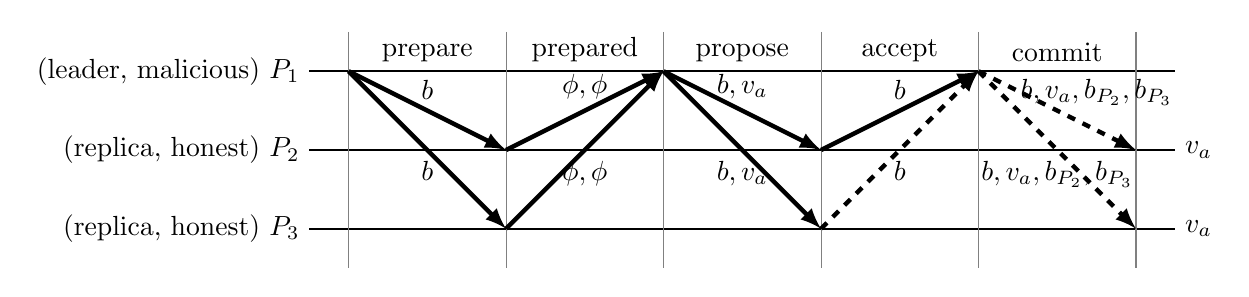
\begin{tikzpicture}[auto]
        % \tikzstyle{every node}=[font=\footnotesize];

        % horizontal line
        \draw[thick] (-0.5,-1) -- (10.5,-1);
        \draw[thick] (-0.5,-2) -- (10.5,-2);
        \draw[thick] (-0.5,-3) -- (10.5,-3);

        % vertical line
        \draw[gray] (0,-0.5) -- (0,-3.5);
        \draw[gray] (2,-0.5) -- (2,-3.5);
        \draw[gray] (4,-0.5) -- (4,-3.5);
        \draw[gray] (6,-0.5) -- (6,-3.5);
        \draw[gray] (8,-0.5) -- (8,-3.5);
        \draw[gray] (10,-0.5) -- (10,-3.5);

        % party start
        \node[anchor=east] at (-0.5,-1) {(leader, malicious) $P_1$};
        \node[anchor=east] at (-0.5,-2) {(replica, honest) $P_2$};
        \node[anchor=east] at (-0.5,-3) {(replica, honest) $P_3$};

        % party end
        \node[anchor=west] at (10.5,-1) {};
        \node[anchor=west] at (10.5,-2) {$v_a$};
        \node[anchor=west] at (10.5,-3) {$v_a$};

        % phase
        \node[anchor=south] at (1,-1) {prepare};
        \node[anchor=south] at (3,-1) {prepared};
        \node[anchor=south] at (5,-1) {propose};
        \node[anchor=south] at (7,-1) {accept};
        \node[anchor=south] at (9,-1) {commit};

        % prepare
        \draw[-latex, ultra thick] (0,-1) -- (2,-2) node [midway,above] {$b$};
        \draw[-latex, ultra thick] (0,-1) -- (2,-3) node [midway,below] {$b$};

        % prepared
        \draw[-latex, ultra thick] (2,-2) -- (4, -1) node [midway,above] {$\phi, \phi$};
        \draw[-latex, ultra thick] (2,-3) -- (4, -1) node [midway,below] {$\phi, \phi$};

        % propose
        \draw[-latex, ultra thick] (4,-1) -- (6,-2) node [midway,above] {$b, v_a$};
        \draw[-latex, ultra thick] (4,-1) -- (6,-3) node [midway,below] {$b, v_a$};

        % accept
        \draw[-latex, ultra thick] (6,-2) -- (8, -1) node [midway,above] {$b$};
        \draw[-latex, ultra thick, dashed] (6,-3) -- (8, -1) node [midway,below] {$b$};

        % commit
        \draw[-latex, ultra thick, dashed] (8,-1) -- (10,-2) node [near end,above=5pt] {$b, v_a, b_{P_2}, b_{P_3}$};
        \draw[-latex, ultra thick, dashed] (8,-1) -- (10,-3) node [midway,below] {$b, v_a, b_{P_2}, b_{P_3}$};
    \end{tikzpicture}
    \label{fig:safety_2_solution}
    \caption{Safety attack 2 solution}
\end{figure}

\end{document}